\chapter{Introduction}\label{ch:introduction}

This operating manual covers the \ReplicaGenOne{} and \ReplicaNextLong{} digital instrument clusters for Volkswagen Golf~II, Jetta~II, and Scirocco~II vehicles. It summarises the hardware variants, describes their functions, and explains how to install, configure, operate, store, and maintain the dashboards. The guidance is intended for vehicle owners, automotive electricians, and service centres that retrofit the product.

The following chapters provide the product identification scheme, connector pin-outs, operating conditions, and detailed installation and configuration procedures. Maintenance and troubleshooting references for both Replica generations are also included so the instrument panel can be serviced without the factory documentation.

\begin{figure}[htbp]
    \centering
    \begin{subfigure}{0.48\textwidth}
        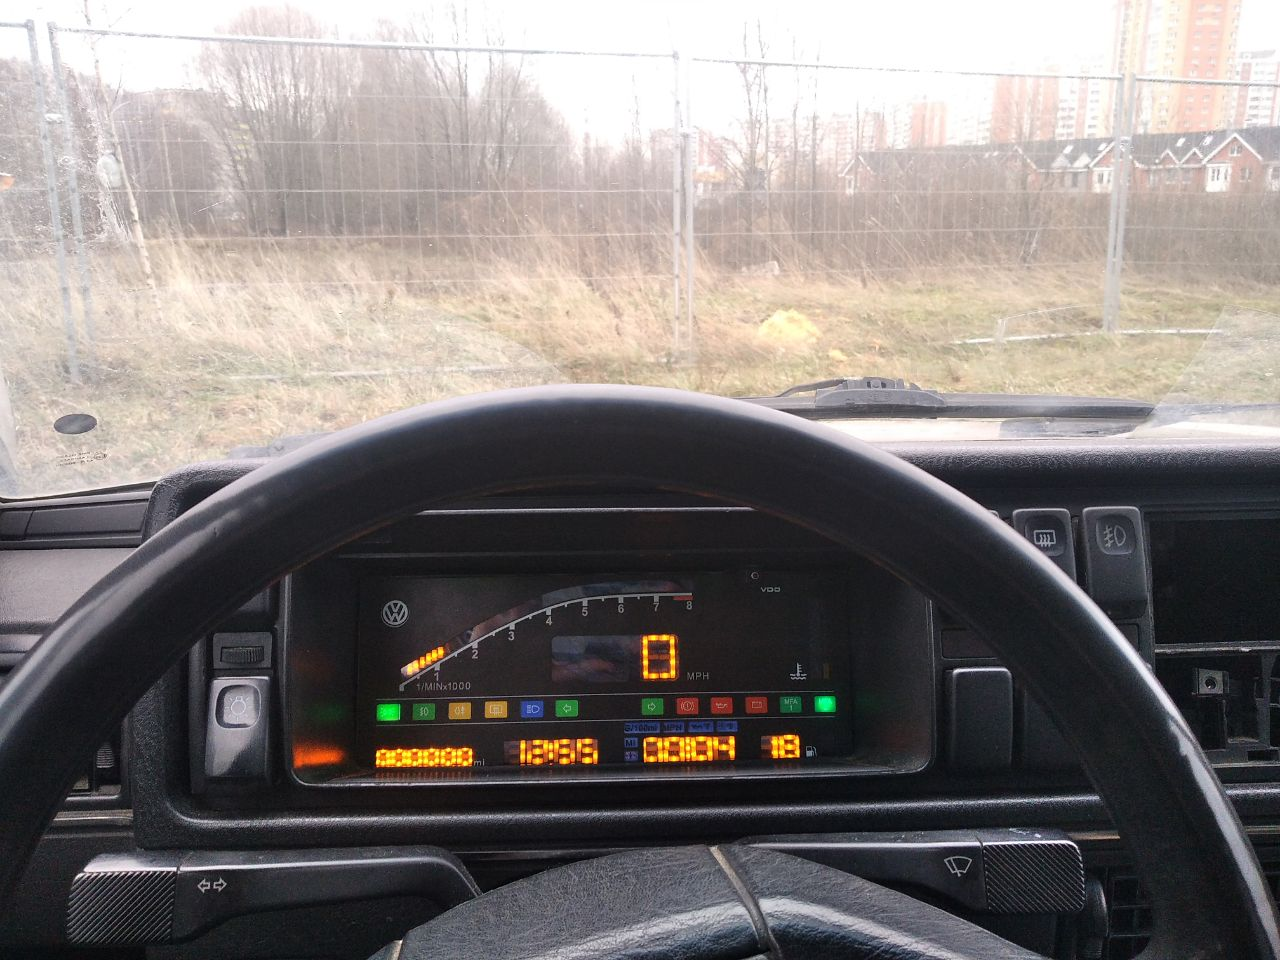
\includegraphics[width=\linewidth]{digifiz_manual/image004.jpg}
        \caption{Delivery set for the GART~8--MGF configuration.}
    \end{subfigure}\hfill
    \begin{subfigure}{0.48\textwidth}
        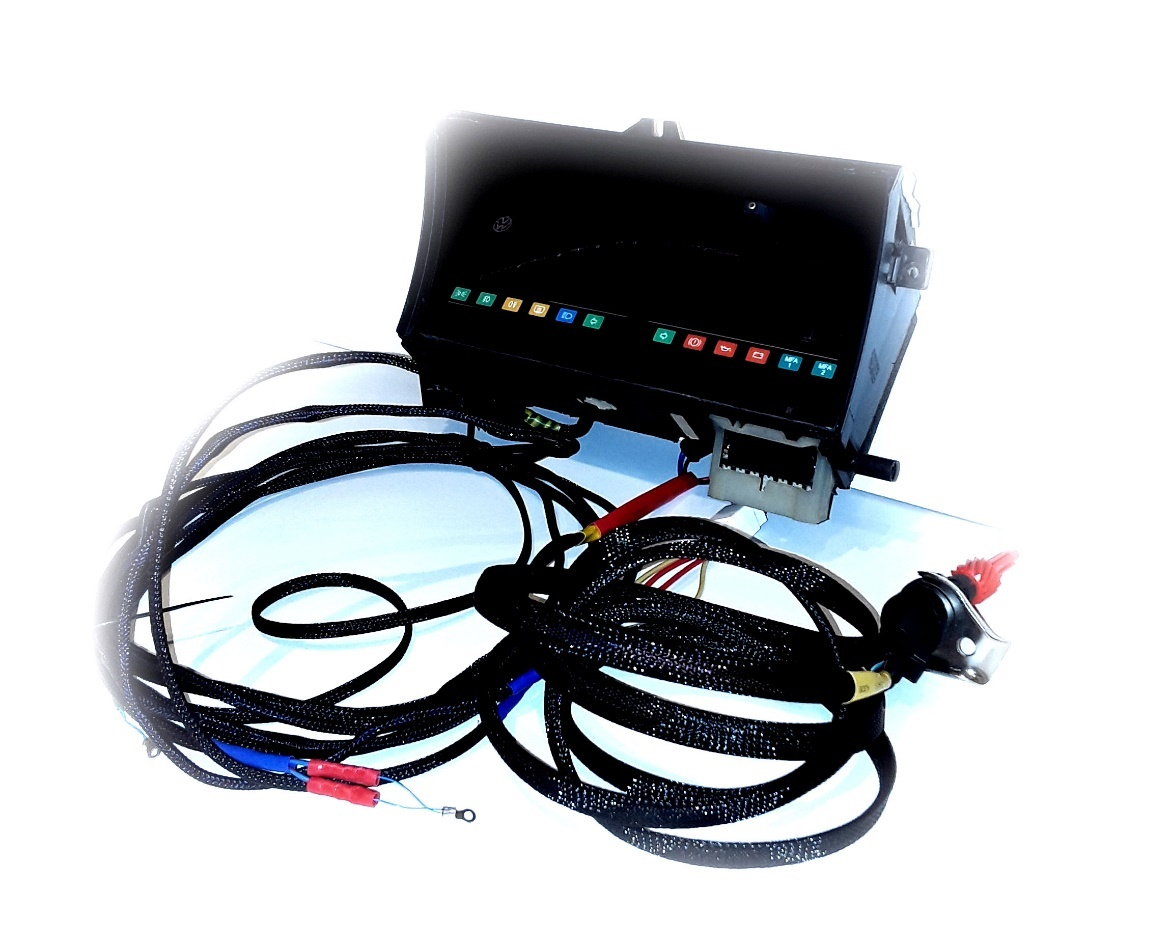
\includegraphics[width=\linewidth]{digifiz_manual/image005.jpg}
        \caption{Typical contents of a GART package.}
    \end{subfigure}
    \begin{subfigure}{0.48\textwidth}
        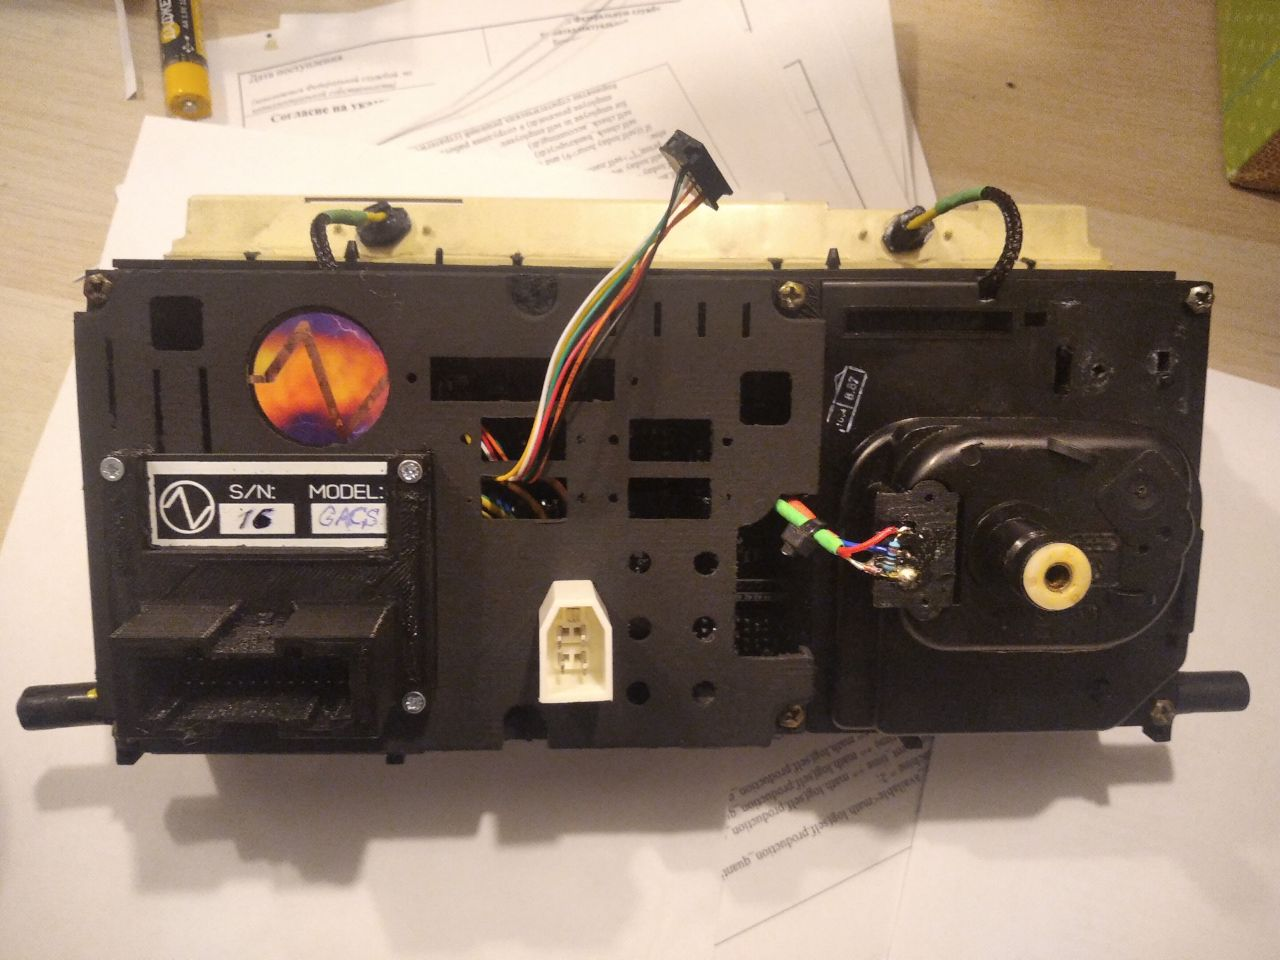
\includegraphics[width=\linewidth]{digifiz_manual/image006.jpg}
        \caption{Rear view of the single-connector GACS assembly.}
    \end{subfigure}\hfill
    \begin{subfigure}{0.48\textwidth}
        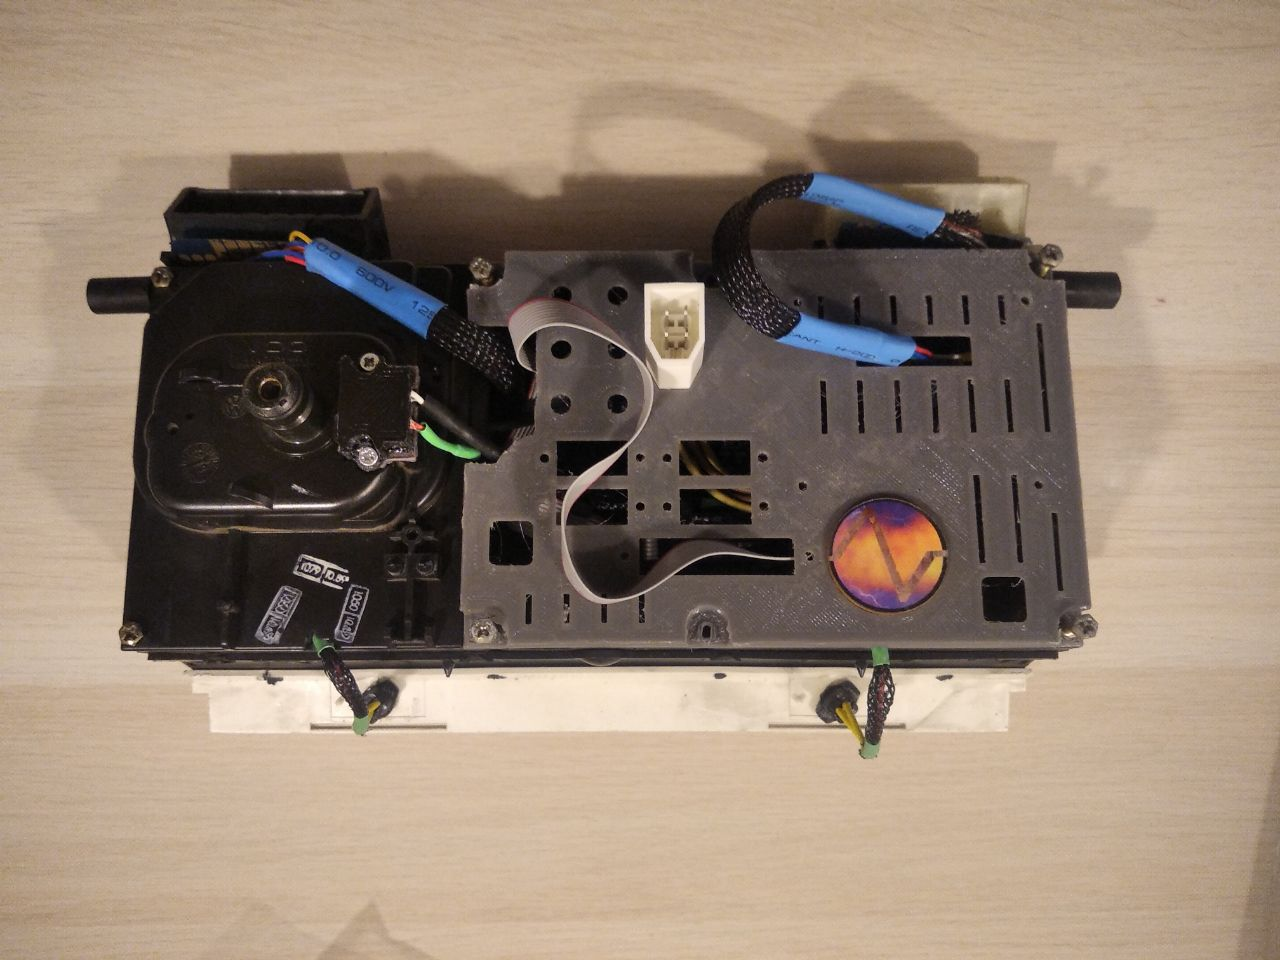
\includegraphics[width=\linewidth]{digifiz_manual/image007.jpg}
        \caption{Rear view of the dual-connector GACT assembly.}
    \end{subfigure}
    \caption{Representative \ReplicaGenOne{} and \ReplicaNextLong{} instrument panels supplied with this manual.}
\end{figure}

Each variant ships with the components required for the intended drivetrain, measurement units, and wiring harness style. Later chapters decode the variant markings and provide connector tables so the cluster can be integrated safely.
